\chapter{Описание моделей, отвечающих за генерацию поведения виртуального актора}


В данном разделе приводится теоретическое описание модели.




\section{Постановка задачи}

В рамках научно-исследовательской работы был выявлен альтернативный путь решения поставленной задачи задачи, который выражается 
в обучения нейронной сети. Данный метод рассматривается параллельно реализации с использованием когнитивной архитектурой eBICA. 
eBICA – “emotional biologically inspired cognitive architecture” – “эмоциональная биологически вдохновленная когнитивная архитектура”. 
В этой архитектуре эмоциональные элементы добавлены практически ко всем процессам за счет модификации основных строительных блоков архитектуры. 
Ключевым моментом этой когнитивной архитектуры являются оценки, которые связаны со схемами и психическими состояниями как их атрибуты, 
моральные схемы, которые контролируют модели оценок и представляют социальные эмоции, а также семантические пространства, которые дают 
значения этих оценок.

Как видно из (Рис. \ref{pic:ris7}), архитектура представляет собой конгломерат компонентов: интерфейсный буфер, рабочая, процедурная, семантическая 
и эпизодическая системы памяти, система ценностей и система когнитивных карт \cite{Samsonovich01}. Три основных строительных блока для этих компонентов - это 
ментальные состояния, схемы и семантические карты. Семантическая память - это коллекция определений схем. Буфер интерфейса заполняется схемами.

\begin{figure}[h]
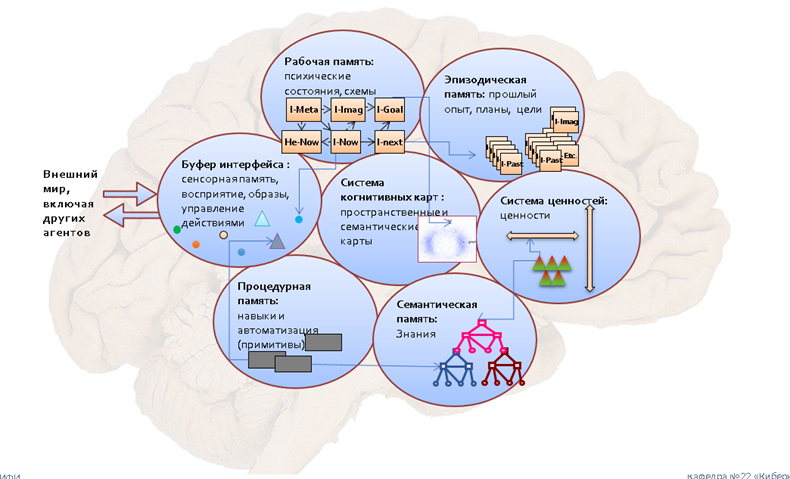
\includegraphics[width=0.75\columnwidth]{./img/ris7.png}
\centering  
\caption{Структура когнитивной архитектуры eBICA}
\label{pic:ris7}
\end{figure}

Рабочая память включает активные психические состояния. Эпизодическая память хранит неактивные психические состояния, сгруппированные 
в эпизоды - предыдущее содержимое рабочей памяти. Следовательно, эпизодическая память состоит из структур, аналогичных тем, которые 
обнаруживаются в рабочей памяти, но которые «заморожены» в долговременной памяти. Процедурная память включает в себя примитивы. Система 
ценностей включает в себя шкалы, представляющие основные значения. Система когнитивных карт включает, в частности, семантические карты 
эмоциональных ценностей. Семантическая карта использует абстрактное метрическое пространство (семантическое пространство) для представления 
семантических отношений между ментальными состояниями, схемами и их экземплярами, а также для присвоения значений их оценкам.

\section{Сбор данных о юморе}
Для обучения нейронной осуществляется сбор данных. Самой частой альтернативой сбора данных является его получение из открытых ресурсов при помощи парсинга кода HTML.

Для парсинга страниц используются несколько основных методов описанных в \cite{parser02}.
\begin{enumerate}
  \item Парсинг получаемого JSON при помощи Api
  \item Парсинг по XHR запросам в консоли разработчика браузера
  \item Поиск JSON в html странице
  \item Рендеринг код страницы через автоматизацию браузера
\end{enumerate}

В частности, используется нейросетевой подход для парсинга данных. Такой подход актуален так как владельцы информационных продуктов 
часто не заинтересованы в том, чтобы пользователи парсили данные с их ресурсов и добавляют различные ограничения и алгоритмы по распознаванию 
парсинга. Самым простым примером является ограничение на количество запросов к сайту, вставка капчи, проверка IP пользователя на соответствие 
региону либо количество посещений страницы в минуту. Так же очень частой проблемой является динамическая доработка сайтов, которая в следствии 
заставляет переделывать алгоритм парсинга.

Для того, чтобы парсинг страниц был более практичным, используют нейросетевой подход. Одним из таких инструментов является TensorFlow, 
это открытая программная библиотека для машинного обучения, разработанная компанией Google для решения задач построения и тренировки 
нейронной сети с целью автоматического нахождения и классификации образов, достигая качества человеческого восприятия. 

Для решения проблемы с IP используют спуфинг, что представляет из себя принцип маскировки одного юнита под другого путём фальсификации 
данных и позволяет получить соответствующие преимущества. 

Для анализа были взяты данные с различных сайтов с юмористическим посылом. В первую очередь рассматривались сайты со скетчами или сценками 
(в том числе скетчи из различных юмористических передач). Для каждого скетча и сценки на сайте должно быть их текстовое описание, поясняющее 
сюжет или сценарий. Далее рассматривались сайты с анекдотами и различными шутками. Такой приоритет был поставлен в связи с тем, что основой 
юмора в клоунаде должны быть действия акторов на сцене, а не юмористический эффект, полученный в результате “игры слов”. 

\section{Предварительная обработка полученных данных}

На вход модели должен подаваться заранее обработанный корпус текстов. Предварительная обработка состоит из следующих этапов \cite{seman06}:

\begin{itemize}
  \item Удаление всех знаков препинания, чисел и слов «нецелевых» языков (не предназначенных для обработки моделью).
  \item Разбиение текста на предложения. Для этого был выбран пакет библиотек Natural Language Toolkit (NLTK). Данная библиотека применяет регулярные выражения, а также некоторые алгоритмы машинного обучения для обработки естественного языка. Базовая версия NLTK не поддерживает разбиение русскоязычных текстов на предложения, поэтому использовалась модификация, расширяющая функционал библиотеки.
  \item Удаление «стоп-слов» – слов, не несущих определенной смысловой нагрузки, но при этом затрудняющих обработку исходного текста. Обычно для каждой специфической задачи применяется свой словарь стоп-слов, однако для нашей задачи достаточно стандартного словаря, содержащего буквы, частицы, предлоги, союзы, местоимения, числительные. Установлено, что удаление стоп-слов из тренировочного набора значительно снижает вычислительную стоимость, а также повышает точность модели.
  \item К корпусу текстов применяется стемминг или лемматизация. Это позволяет сократить размер словаря и искать семантически близкие слова, а не разные формы одного слова. Стемминг – это поиск основы слова, причем не обязательно совпадающей с корнем. Он имеет высокую скорость работы, но наиболее эффективен для английского языка, так как в нем для нахождения основы слова обычно достаточно удалить окончание. Для русского языка стемминг малоэффективен, поэтому применяется более ресурсоемкий алгоритм лемматизации. Лемматизация – это процесс приведения слова к начальной форме. В данной работе лемматизация осуществлялась морфологическим анализатором MyStem .
  \item Дополнение предложений до одинаковой длины с использованием нейтрального слова, так как сверточные нейронные сети способны обрабатывать только последовательности одинаковой длины.
\end{itemize}

Далее на начальном этапе необходимо перевести слова естественного языка в форму, пригодную для анализа сверточной нейронной сетью. 
Для этого лучше всего подходит векторное представление слов. Кроме того, среди всех моделей выберем ту, которая наиболее точно отражает 
реальные взаимосвязи между словами, а именно семантическую близость. Отметим, что модель не должна быть слишком требовательной к вычислительным 
ресурсам, чтобы было возможно совершать обучение сети на достаточно больших объемах данных.

Для выявления семантических связей между словами воспользуемся предположением лингвистики – 
дистрибутивной гипотезой: лингвистические единицы, встречающиеся в схожих контекстах, имеют близкие значения. 
Во многих моделях обработки текстов входные данные кодируются унарным кодом (one-hotencoding) – вектором, размерность которого равна мощности словаря более подробно 
описанный в \cite{neural02}. Элемент, соответствующий И.А. Батраева, А.Д. Нарцев, А.С. Лезгян номеру слова в словаре, равен единице, а остальные элементы равны нулю.
Однако у этого метода, согласно \cite{neural02} есть ряд существенных недостатков:

\begin{itemize}
  \item словари естественных языков могут быть достаточно объемными и исчисляться десятками и сотнями тысяч слов; следовательно, если каждое слово кодировать таким вектором, объем данных становится слишком большим;
  \item при таком способе кодирования теряется связь между словами: все слова считаются разными и никак не связанными между собой.
\end{itemize}

В силу вышесказанного, one-hot encoding не подходит для анализа семантической близостислов. Поэтому для данной задачи воспользуемся другим способом кодирования – распределенным представлением слов.
Распределенное (или векторное) представление слов – это способ представления слов в виде векторов евклидова пространства, размерность которого обычно равна нескольким сотням. Основная идея заключается в том, что геометрические отношения между точками евклидова пространства будут соответствовать семантическим отношениям между словами. Например, слова, представленные двумя близко расположенными точками векторного пространства, будут, скорее всего, синонимами или просто тесно связанными по смыслу словами. Семантическая близость слов вычисляется как расстояние между векторами, для чего используется так называемая косинусная мера.

Word2vec включает в себя две различные архитектуры – CBOW (Continuous Bag of Words – непрерывный мешок слов) и Skip-gram \cite{seman01}. CBOW пытается предсказать слово, исходя из текущего контекста, а Skip-gram, наоборот, пытается предсказать контекст по текущему слову. Для реализации модели была выбрана архитектура Skip-gram, которая, несмотря на меньшую скорость обучения, лучше работает с редкими словами.
Предварительно обработанный текст можно подавать на вход модели, после чего будут выполнены следующие действия:

\begin{itemize}
  \item считывается корпус текстов и рассчитывается, сколько раз в нем встретилось каждое слово; 
  \item из этих слов формируется словарь, который сортируется по частоте слов; также из словаря
  \item для сокращения его размера удаляются редкие слова;
  \item модель идет по субпредложению (обычно предложение исходного текста или абзац) окном определенного размера; под размером окна понимается максимальная длина между текущим словом и словом, которое предсказывается. Оптимальный размер окна – 10 слов; 
  \item	к данным, находящимся в текущем окне, применяется нейронная сеть прямого распространения с линейной функцией активации скрытого слоя и функцией активации softmax для выходного слоя.
\end{itemize}

Из всего вышесказанного ясно, что матрицы, задающие скрытый и выходной слои, получаются чрезвычайно большими. 
Это делает обучение сети долгим процессом. Поэтому используются различные оптимизации, которые позволяют существенно 
снизить, согласно \cite{neural03} временные и вычислительные затраты, незначительно потеряв в точности. Одной из таких модификаций является субсемплирование.
Чтобы избежать дисбаланса между редкими и часто встречающимися словами, используется простой подход: каждое слово 
отбрасывается с вероятностью, зависящей от частоты вхождения этого слова в текст.

\section{Описание работы модели актора в старом приложении}

На момент начала выполнения работы уже была реализована система работы виртуальных агентов, и она состоит в том, что сперва 
считываются действия и объекты с заданными для них параметрами и значениями из Excel файла, а также инициализируются значения. 
Затем выбор действий происходит в следующем порядке: в радиусе вокруг оценок виртуального актора выбираются действия, которые 
попадают в этот радиус, а также проверяются различные условия, необходимые для выполнения действия. Если условия не выполняются, 
то действие не может быть выбрано. Затем, после того как в список добавлены все действия, которые могут быть выполнены, рассчитываются 
вероятности на основе оценок и рассчитанных констант. Также, если действие повторное, его вероятность несколько занижается. 
После расчета вероятностей выбирается действие, которое влияет на оценки самого клоуна, а также, если есть, на цель клоуна. 

Помимо этого происходит замена состояний объектов и виртуальных акторов. После этого происходит перерасчет оценок Appraisals и Feelings \cite{Samsonovich01}.

Основная модель eBICA определяет поведение виртуального актора исходя из следующих факторов:

\begin{itemize}
  \item соматический;
  \item рациональный;
  \item когнитивный.
\end{itemize}

Нравственный фактор регулирует отношения первого актора со вторым на основе системы ценностей (представленной семантической картой) 
и моральных схем. Под когнитивным фактором понимается учет соображений нравственности, этики и морали, общей системы ценностей, 
понятий о добре и зле, о собственном достоинстве, эмпатии, соображений эстетики, стремлений к простоте и элегантности, и т.д. 
Учет этих соображений возможен на основе когнитивных оценок (appraisals) всех релевантных агентов, событий, их возможных действий 
и последствий этих действий, фактов, свойств, отношений, и т.д. Возможен вариант модели, в которой ответное действие может выбираться 
лишь из двух вариантов: положительная реакция на действие человека и отрицательная. Данная версия модели весьма неплохо работает даже 
с таким ограничением. Но невозможно придерживаться данной парадигмы при увеличении количества возможных вариантов для взаимодействия 
между акторами. В данной модели необходимо учесть пересчет оценок Appraisals и Feelings. Для пересчета оценок Appraisals используется 
следующая формула \ref{eq:appraisals01}:

\begin{equation}
  \begin{gathered}
    Appraisals=(1-r)*Appraisals+r*Action
    %P_{i+1j  } (R_{i+1j  } , {\varphi}_{i+1} , {\theta}_{j  }) \\
  \end{gathered}
  \label{eq:appraisals01}
\end{equation}

где Appraisals - оценка, 
r - эмпирически вычисленная константа экспоненциального затухания, 
Action - оценка совершаемого действия на семантической карте.

Одновременно с Appraisals пересчитываются так называемые “чувства” Feelings согласно режиму работы моральной схемы.
Аффективное пространство VAD – это трехмерное векторное пространство, точки которого соответствуют определенным эмоциональным 
состояниям, или аффектам, представленным триплетами значений (Valence, Arousal, Dominance). 
Существуют и сходные модели: PAD (Pleasure, Arousal, Dominance), EPA (Evaluation, Potency, Arousal) и другие. 
Здесь мы используем модель VAD. Соответственно, под «семантической картой» здесь часто понимается ее конкретная 
разновидность: аффективная карта (или когнитивная семантическая карта).

Шкалы имеют следующие значения:
\begin{itemize}
  \item dominance – варьируется при значении от 0 (покорность) до +1 (доминантность) и описывает соответствующие чувства; 
  \item valense – при значениях от -1 до 0 показывает уровень негатива или радости соответственно; 
  \item arousal – значения от -1 до 1 показывают уровень возбуждения (заинтересованности), к примеру, гнев по уровню возбуждения сильнее раздражительности, но слабее ярости. 
\end{itemize}

Оценки представлены в виде векторов на трехмерной семантической карте \cite{seman_karta}, \ref{pic:ris5}.
Моральная схема определяет общую установку на оценку поведения акторов, согласно их ролям и типу ситуации. 
Ее целью (как агента) является достижение и поддержание «нормального» положения дел, определенного набором Feelings. 
Вообще говоря, моральная схема состоит из двух частей: части, распознающей тип ситуации и осуществляющей привязку (binding),
и части, реализующей динамику схемы. В случае парадигмы актора можно считать, что моральная схема одна, уже привязана, и 
потому первая часть ее не актуальна.

Субъективные оценки (Feelings) генерируются по определенным правилам на основании истории объективных оценок и состояний системы. 
Грубо говоря, Feelings – это субъективное представление о том, каким оцениваемый актор является «на самом деле», и, следовательно, 
какого поведения от него нужно ожидать и на какое место его нужно ставить своим поведением. Следовательно, выбор поведения актора 
должен осуществляться так, чтобы приблизить Appraisals к Feelings. 

Значение Feelings определяет моральная схема, которая может работать в одном из трех режимов. 
Первый режим основывается на формуле \ref{eq:feelings01}:

\begin{equation}
  \begin{gathered}
    Feelings=beta*Appraisals
  \end{gathered}
  \label{eq:feelings01}
\end{equation}

где beta – эмпирически вычисленная константа. 

В данном режиме схема говорит, что если актор ведет себя хорошо, то к нему нужно относиться как к хорошему, и т.д. 

Цель данного процесса – распознать и классифицировать актора, выработать отношение к нему и приписать ему определенную роль во взаимоотношениях. 

В данном режиме моральная схема работает пока разница между квадратами норм Feeling и Appraisals не станет меньше некоторого значения.

Суть второго режима заключается в том, что значение Feeling фиксировано и экстремально по абсолютной величине, т.е. находится на сфере, 
ограничивающей семантическую карту (предположим, что есть такая сфера). Направленность вектора Feeling может быть либо произвольной, 
определенной предысторией, либо дискретной – вдоль одной из осей.

Третий режим состоит в том, что значения Feelings меняются \ref{eq:feelings02}, подстраиваясь под текущие значения Appraisals (здесь r1 может быть отличным от r): 

\begin{equation}
  \begin{gathered}
    Feelings=(1-r_1 )*Feelings+r1*(Appraisal-Feelings)
  \end{gathered}
  \label{eq:feelings02}
\end{equation}

Соответственно значения Appraisals и Feelings как говорится в работе \cite{Samsonovich05} пересчитываются после каждого действия первого актора, направленного на второго актора.
Также пересчет оценок происходит после определения и совершения одним из акторов ответного или самостоятельного действия. 
В данном контексте под термином “самостоятельное действие” имеется в виду действие, основанное лишь на текущем состоянии мира и 
значений векторов Appraisals и Feelings акторов, отобрежнные на (Рис. \ref{pic:ris8}). 


\begin{figure}[h]
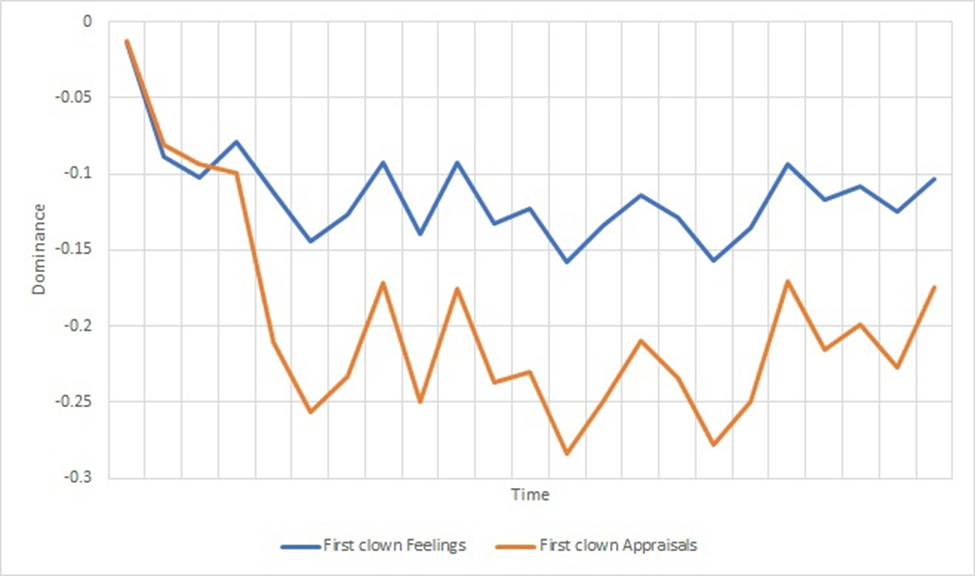
\includegraphics[width=0.75\columnwidth]{./img/ris8.png}
\centering
\caption{Корреляция значений Appraisals (оранжевая) и Feelings (синяя) для показателя доминантности на протяжении времени/действий с шагом в 5 секунд}
\label{pic:ris8}
\end{figure}

Согласно (Рис. \ref{pic:ris8}) мы видим, что работа модели сводится к выбору действия, 
которое будет максимально приближать Appraisals к Feelings и вектор соматического состояния к начальному положению.

\section{Рекуррентные нейронные сети}

LSTM — это класс возвратных нейронных сетей. Поэтому, прежде чем мы сможем перейти к LSTM, 
важно понять нейронные сети и рекуррентные нейронные сети \cite{Wikipedia01}. 

Нейронные сети - Искусственная нейронная сеть представляет собой слоистую структуру из связанных нейронов,
вдохновленную биологическими нейронными сетями. Это не один алгоритм, а комбинация различных алгоритмов, 
которая позволяет нам выполнять сложные операции с данными. 
Рекуррентные нейронные сети - это класс нейронных сетей, предназначенных для работы с временными данными. 
Нейроны RNN имеют состояние / память ячейки, и ввод обрабатывается в соответствии 
с этим внутренним состоянием, которое достигается с помощью петель в нейронной сети. 
В RNN существуют повторяющиеся модули «tanh» слоев, которые позволяют им сохранять информацию. 
Однако ненадолго, поэтому нам нужны модели LSTM. 

LSTM - Это особый вид рекуррентной нейронной сети, способной изучать долгосрочные зависимости в данных. 
Это достигается за счет того, что повторяющийся модуль модели имеет комбинацию четырех слоев, взаимодействующих друг с другом \cite{Wikipedia01}. 

На (Рис. \ref{pic:ris9}) отображены структуры вышеупомянутые виды рекуррентных сетей: 

\begin{figure}[h]
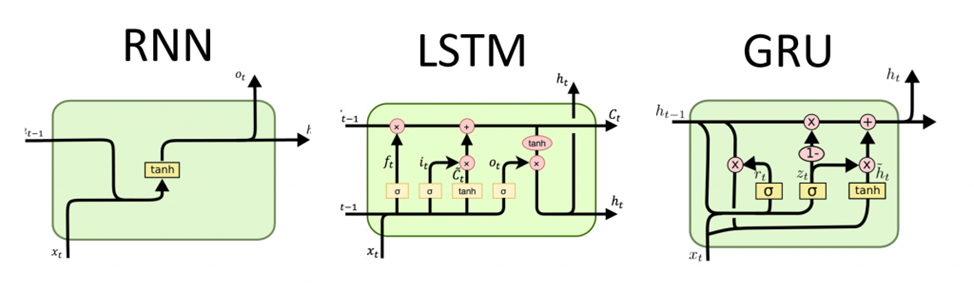
\includegraphics[width=0.75\columnwidth]{./img/ris9.png}
\centering
\caption{Структуры рекуррентных нейронных сетей}
\label{pic:ris9}
\end{figure}

\section{Выводы}

В данном разделе была сформулирована постановка задачи, рассмотрены возможные ее решения с помощью архитектуры eBICA и нейронных сетей. 
Обозначена проблема сбора данных для обучения нейронной сети с веб-сервисов, и были выявлены способы решения данной проблемы. 
А также рассмотрена проблема обработки данных применительно к модели действий виртуальных агентов. Обозначены основные положения 
поведения виртуальных агентов. Выбран вид нейронной сети, которая будет моделировать поведение виртуальных акторов, а именно 
рекуррентная нейронная сеть.
